\documentclass[10pt]{article}
%\usepackage[margin=1in]{geometry}
\usepackage{amsmath,amssymb,graphicx}
\usepackage{hyperref}
\setlength\parindent{0pt}
\begin{document}
\title{Assignment 1: Sparse Matrices}
\author{1212550}
\begin{center}
\section*{Assignment 1: Sparse Matrices}


The following is a brief report concerning the implementation\\ of my class $\textit{Sparse.cc}$ upon specific matrices.\\
\end{center}

\section{The Gauss Seidel Algorithm}

The  $\textit{Gauss Seidel}$  algorithm is a Splitting method used to solve a system of linear equations, which we represent in matrix form as $Ax=b$. A Splitting method has the general form
\[ Px^{(k+1)} = Nx^{(k)} + b, \]
where $A = P - N$ is the matrix splitting. This is equivalent to
\[ x^{(k+1)} = x^{(k)} + P^{-1}r^{(k)}, \]
where $r^{(k)} = b - Ax^{(k)}$ is called the residual. For the implementation of this method we redifine our decomposition of $A$ to be $A = D - (E+F)$, where $-E,D,-F$ are the lower triangular matrix, diagonal matrix and upper triangular matrix of $A$ respectively. For the $\textit{Gauss Seidel}$ method itself, $P = D - E$ and $N = F$. The convergence of iterations of this type depends on the spectral radius $\rho(P^{-1}N)$, where
\[ \rho(A) = \text{max}\{ |\lambda|: \lambda \in \lambda(A) \}. \]
The $\textit{Gauss Seidel}$ method can be applied to any matrix with non-zero elements on the diagonals, but convergence is only guaranteed if the matrix is either diagonally dominant, or symmetric and positive definite. \\

Noting that the matrix $P$ is in triangular form, and
\[ x^{(k+1)} = P^{-1}(Nx^{(k)} + b),\]
the elements $x^{(k+1)}$ can be computed using forward substitution. Thus it follows that
\[ x_i^{(k+1)} = \frac{1}{a_{ii}} \Big( b_i - \sum_{j=1}^{i-1}x^{(k+1)}a_{ij} - \sum_{j=i+1}^{n}x^{(k)}a_{ij} \Big), \]
for $i = 1,...,n$. The procedure continues until the residual error, defined by $||r^{(k)}|| = ||b- A x^{(k)}||$, is below some tolerance or the algorithm has stagnated. For the implementation used in this assignment, the norm is the $L^{\infty}$ norm. Note that elements of the approximation $x^{(k)}$ can be overwritten in this algorithm, so only one storage vector for the approximation will be needed in practice. \\

For this assignment I have implemented a sparse matrix class called $\textit{Sparse.cc}$, which let the user store matrices in row major format in such a way that only non-zero elements are stored in memory. It contains a member function which allows the user to add entries to a blank matrix of their choice dimensions, along with other useful functions. In particular, it has a member function called $\textit{GaussSeidel}$, which, for an initial guess $x^{(0)}$ and input vector $b$, performs the above algorithm and returns a vector of two vectors. The first vector is the approximated solution and the second vector contains the residual error for each iteration. This will implicitly return the number of iterations computed, since it will be equal to the size of the second vector.\\

I have set the function such that it continues iterating as long as the residual error for each iteration is above a tolerance of $1e - 6$ and no more than $500,000$ iterations have been computed. Furthermore, the function checks that the input vectors are of appropriate dimension and that the diagonal of the matrix is non-zero. If any of these errors occur, the returned vector contains the residual error between $b$ and $x^{(0)}$ only. A warning stating this is issued to the user in these cases.

\section{Testing the Algorithm}
I have tested my implementation for a matrix $A \in \mathbb{R}^{N \times N}$ and vector $b \in \mathbb{R}^N$ defined as follows for $i,j = 0,...,N-1$:

$$a_{ij}=
\begin{cases}
-D_i &\text{for} \quad j = i-1\\
D_i + D_{i-1} &\text{for} \quad j=i\\
-D_{i} &\text{for} \quad j = i + 1\\
0 &\text{otherwise}
\end{cases}
$$
where $D_i=a(w_i - \frac{1}{2})^2 + \delta$, $w_i = \frac{i+1}{N+1}$ for constants $a=(4-\delta)$, $\delta > 0$, and
$$b_{i}=
\begin{cases}
-2a(w_i - \frac{1}{2})w_0^2 &\text{for} \quad i = 0,...,N-2\\
-2a(w_i - \frac{1}{2})w_0^2 + 1 &\text{for} \quad i=N-1.
\end{cases}
$$

\subsection{Varying the Dimension}
Initially $\delta$ was set to be $1$, and I tested the method for $N=100$, $1000$, and $100000$. As N increased, the computation took longer, and altering the code to improve efficiency was needed in order to run the $N=10000$ case. Nevertheless, this computation now runs within two minutes. Noting that for $\delta = 1$, the exact solution is given by $(w_i)_{i=1}^{N-1}$, it was possible to compute the error between the outputted approximation and the true solution. This was done using the $L^\infty$ norm and the results can be seen in the following table. It contains the number of iterations computed, the $\textit{Residual Error}$ (the final residual error calculated before terminating the algorithm), and the $\textit{Error}$ (the error between the approximated solution and true solution).

\begin{center}
 \begin{tabular}{||c c c c ||}
 \hline
 N & Iterations & Residual Error & Error \\ [0.5ex]
 \hline\hline
 100 & 6664 & 9.99475e-07 & 0.001032 \\
 \hline
 1000 & 186647 & 9.99996e-07 & 0.101512  \\
 \hline
 10000 & 242319 & 9.99999e-07 & 0.819303 \\
 \hline
\end{tabular}
\end{center}

\subsection{Varying $\delta$ for Fixed Dimension}
I then fixed the dimension $N$ to be $100$ and the method was implemented for $\delta$ equalling $0.01,0.1,1,10$ and $100$. Data from these implementations can be seen in the following table.

\begin{center}
 \begin{tabular}{||c c c ||}
 \hline
 $\delta$ & Iterations & Residual Error \\ [0.5ex]
 \hline\hline
 0.01 & 1825 & 9.98327e-07  \\
 \hline
 0.1 & 2536 & 9.99553e-07  \\
 \hline
 1 & 6664 & 9.99475e-07 \\
 \hline
 10 & 17137 & 9.99929e-07 \\
 \hline
 100 & 27419 & 9.99763e-07 \\
 \hline
\end{tabular}
\end{center}
Furthermore, I plotted the residual error at each iteration for these values of $\delta$ in a log-log scale graph, which can be seen in figure~\ref{fig:func_and_deriv}.
Clearly the number of iterations needed for the approximation to be within tolerance increases as $\delta$ increases. This is due to the maximum eigenvalue of $P^{-1}N$ increasing as $\delta$ increases, which increases the spectral radius $\rho(P^{-1}N)$ and thus affects the rate of convergence.

\subsection{Adding a Diagonal Matrix}
For the next test, $N$ was fixed as $100$ and $\delta$ fixed as $1$. This test was implemented to see the effect of replacing the matrix $A$ in the Gauss Seidel implementation with the matrix $A+\lambda I$, for some $\lambda \in \mathbb{R}^+$. I tested the implementation for $\lambda$ equalling $0.01,0.1,1,10$ and $100$. Data from these implementations can bee seen in the following table.
\begin{center}
 \begin{tabular}{||c c c ||}
 \hline
 $\lambda$ & Iterations & Residual Error \\ [0.5ex]
 \hline\hline
 0.01 & 620 & 9.94105e-07  \\
 \hline
 0.1 & 90 & 9.48631e-07  \\
 \hline
 1 & 17 & 5.12825e-07 \\
 \hline
 10 & 6 & 3.34898e-07 \\
 \hline
 100 & 3 & 9.42322e-07 \\
 \hline
\end{tabular}
\end{center}

The residual error at each iteration was plotted for these values of $\lambda$ in a log-log scale graph, and can be seen in figure figure~\ref{fig:func2}. Note that the condition number for the method is equal to $\frac{\lambda_{\text{max}}}{\lambda_{\text{min}}}$, where $\lambda_\text{max}$ and $\lambda_\text{min}$ are the maximum and minimum eigenvalues of $A$ respectively. Since $\lambda_\text{max} \geq \lambda_\text{min}$, we have that
\[\frac{\lambda_{\text{max}}+c}{\lambda_{\text{min}}+c} \leq \frac{\lambda_{\text{max}}}{\lambda_{\text{min}}},\]
for any $c>0$. Therefore, by adding the matrix $\lambda I$ for $\lambda \in \mathbb{R}^+$ to $A$, we are lowering the condition number. \\

Furthermore, since $A = P - N$, where $P$ is the lower triangular matrix (including diagonal) of $A$, adding the $\lambda I$ directly increases the eigenvalues of $P$ (it does not affect the eigenvalues of $N$). This has the effect of lowering the maximum eigenvalue of $P^{-1}N$ and thus decreases the spectral radius $\rho(P^{-1}N)$, causing the method to converge faster. This agrees with what can bee seen in figure~\ref{fig:func2}.

\clearpage

 \begin{figure}
 \begin{center}
    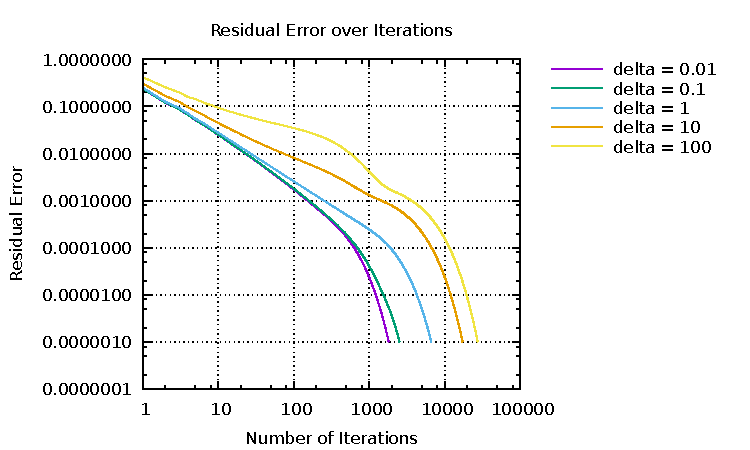
\includegraphics[width=1\textwidth]{function}
  \end{center}
  \caption{As $\delta$ increases the rate of convergence decreases.
  \label{fig:func_and_deriv}}
\end{figure}


\end{document}
